% -*- coding: utf-8; -*-
% vim: set fileencoding=utf-8 :
\documentclass[english,submission]{programming}
%% First parameter: the language is 'english'.
%% Second parameter: use 'submission' for initial submission, remove it for camera-ready (see 5.1)

\usepackage[backend=biber]{biblatex}
\addbibresource{reference.bib}
\usepackage{tikz}
\usepackage{listings}
\usepackage{graphicx}
\usepackage{subcaption} % For subfigures


%
% Packages and Commands specific to article (see 3)
%
% These ones  are used in the guide, replace with your own.
% 
\usepackage{multicol}
\lstdefinelanguage[programming]{TeX}[AlLaTeX]{TeX}{%
  deletetexcs={title,author,bibliography},%
  deletekeywords={tabular},
  morekeywords={abstract},%
  moretexcs={chapter},%
  moretexcs=[2]{title,author,subtitle,keywords,maketitle,titlerunning,authorinfo,affiliation,authorrunning,paperdetails,acks,email},
  moretexcs=[3]{addbibresource,printbibliography,bibliography},%
}%
\lstset{%
  language={[programming]TeX},%
  keywordstyle=\firamedium,
  stringstyle=\color{RosyBrown},%
  texcsstyle=*{\color{Purple}\mdseries},%
  texcsstyle=*[2]{\color{Blue1}},%
  texcsstyle=*[3]{\color{ForestGreen}},%
  commentstyle={\color{FireBrick}},%
}

\newcommand*{\CTAN}[1]{\href{http://ctan.org/tex-archive/#1}{\nolinkurl{CTAN:#1}}}
%%


%%%%%%%%%%%%%%%%%%
%% These data MUST be filled for your submission. (see 5.3)
\paperdetails{
  %% perspective options are: art, sciencetheoretical, scienceempirical, engineering.
  %% Choose exactly the one that best describes this work. (see 2.1)
  perspective=art,
  %% State one or more areas, separated by a comma. (see 2.2)
  %% Please see list of areas in http://programming-journal.org/cfp/
  %% The list is open-ended, so use other areas if yours is/are not listed.
  area={Social Coding, General-purpose programming},
  %% You may choose the license for your paper (see 3.)
  %% License options include: cc-by (default), cc-by-nc
  % license=cc-by,
}
%%%%%%%%%%%%%%%%%%

%%%%%%%%%%%%%%%%%%
%% These data are provided by the editors. May be left out on submission.
%\paperdetails{
%  submitted=2016-08-10,
%  published=2016-10-11,
%  year=2016,
%  volume=1,
%  issue=1,
%  articlenumber=1,
%}
%%%%%%%%%%%%%%%%%%
\definecolor{codegray}{gray}{0.9}
\newcommand{\code}[1]{\colorbox{codegray}{\texttt{#1}}}

\begin{document}

\title{Live probes for free}
%\subtitle{Preparing Articles for Programming}% optional
%\titlerunning{Preparing Articles for Programming} %optional, in case that the title is too long; the running title should fit into the top page column

\author[a]{Jean-Baptiste Döderlein}
\affiliation[a]{ENS Rennes, Bruz, France}
\author[b]{Tijs van der Storm}
\affiliation[b]{CWI, Amsterdam, The Netherlands}
\author[b]{Riemer van Rozen}


\keywords{programming journal, paper formatting, submission preparation} % please provide 1--5 keywords


%%%%%%%%%%%%%%%%%%%%%%%%%%%%%
% Please go to https://dl.acm.org/ccs/ccs.cfm and generate your Classification
% System [view CCS TeX Code] stanz and copy _all of it_ to this place.
%% From HERE
\begin{CCSXML}
<ccs2012>
<concept>
<concept_id>10002944.10011122.10003459</concept_id>
<concept_desc>General and reference~Computing standards, RFCs and guidelines</concept_desc>
<concept_significance>300</concept_significance>
</concept>
<concept>
<concept_id>10010405.10010476.10010477</concept_id>
<concept_desc>Applied computing~Publishing</concept_desc>
<concept_significance>300</concept_significance>
</concept>
</ccs2012>
\end{CCSXML}

\ccsdesc[300]{General and reference~Computing standards, RFCs and guidelines}
\ccsdesc[500]{Applied computing~Publishing}

% To HERE
%%%%%%%%%%%%%%%%%%%%%%%

\maketitle

% Please always include the abstract.
% The abstract MUST be written according to the directives stated in 
% http://programming-journal.org/submission/
% Failure to adhere to the abstract directives may result in the paper
% being returned to the authors.
\begin{abstract}
  %What is the broad context of the work? What is the importance of the general research area?
  \emph{Context}
  In his presentation "Inventing on Principles", Bret Victor demonstrates a live code editor: by specifying input values for a function, we can observe in real time the values taken by the variables during execution, as the code is written. 
  This information is often obtained using a language designed for live programming or by instrumentation of a specific runtime.
  % What problem or question does the paper address? How has this problem or question been addressed by others (if at all)?
  \emph{Inquiry}
  \dots
  % What was done that unveiled new knowledge?
  \emph{Approach}
  In this paper we propose to exploit the capabilities of debuggers to obtain the data needed to design a live code editor.
  % What new facts were uncovered? If the research was not results oriented, what new capabilities are enabled by the work?
  \emph{Knowledge}
  \dots
  % What argument, feasibility proof, artifacts, or results and evaluation support this work?
  \emph{Grounding}
  \dots
  % Why does this work matter?
  \emph{Importance}
  \dots
 
\end{abstract}
\section{Introduction}
\label{sec:introduction}

\section{Problem Overview}
\label{sec:problem-overview}

\section{Using the Debugger ?}
\label{sec:stack-recording}

\subsection{Stack Recording}

\begin{figure}[h]
  \centering
  \begin{minipage}{0.2\textwidth}
    \begin{lstlisting}[language=C]
//foo(3)
int foo(int n) {
  int i = 0;
  while (i < n) {
    i++;
  }
  return i;
}
    \end{lstlisting}
  \end{minipage}
  \hfill
  \begin{minipage}{0.7\textwidth}
    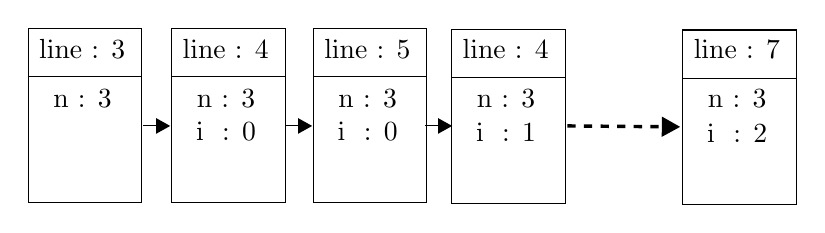
\begin{tikzpicture}[x=0.75pt,y=0.75pt,yscale=-1.1,xscale=0.95]
      
%Shape: Rectangle [id:dp48530454252997635] 
\draw   (11,13.3) -- (68.6,13.3) -- (68.6,34.5) -- (11,34.5) -- cycle ;
%Shape: Rectangle [id:dp4741172814816692] 
\draw   (11,34.5) -- (68.6,34.5) -- (68.6,89.7) -- (11,89.7) -- cycle ;
%Shape: Rectangle [id:dp39333640528563685] 
\draw   (83.8,13.3) -- (141.4,13.3) -- (141.4,34.5) -- (83.8,34.5) -- cycle ;
%Shape: Rectangle [id:dp852338699133017] 
\draw   (83.8,34.5) -- (141.4,34.5) -- (141.4,89.7) -- (83.8,89.7) -- cycle ;
%Shape: Rectangle [id:dp7978026394194542] 
\draw   (155.6,13.3) -- (213.2,13.3) -- (213.2,34.5) -- (155.6,34.5) -- cycle ;
%Shape: Rectangle [id:dp7423976709217543] 
\draw   (155.6,34.5) -- (213.2,34.5) -- (213.2,89.7) -- (155.6,89.7) -- cycle ;
%Shape: Rectangle [id:dp7923849318907303] 
\draw   (225.8,13.7) -- (283.4,13.7) -- (283.4,34.9) -- (225.8,34.9) -- cycle ;
%Shape: Rectangle [id:dp8325747263531937] 
\draw   (225.8,34.9) -- (283.4,34.9) -- (283.4,90.1) -- (225.8,90.1) -- cycle ;
%Shape: Rectangle [id:dp3066063334990279] 
\draw   (343,14.1) -- (400.6,14.1) -- (400.6,35.3) -- (343,35.3) -- cycle ;
%Shape: Rectangle [id:dp9425547748588214] 
\draw   (343,35.3) -- (400.6,35.3) -- (400.6,90.5) -- (343,90.5) -- cycle ;
%Straight Lines [id:da5537198175803346] 
\draw    (69.4,56.1) -- (80,56.1) ;
\draw [shift={(83,56.1)}, rotate = 180] [fill={rgb, 255:red, 0; green, 0; blue, 0 }  ][line width=0.08]  [draw opacity=0] (7.14,-3.43) -- (0,0) -- (7.14,3.43) -- cycle    ;
%Straight Lines [id:da9992180079914922] 
\draw    (141.4,56.1) -- (152,56.1) ;
\draw [shift={(155,56.1)}, rotate = 180] [fill={rgb, 255:red, 0; green, 0; blue, 0 }  ][line width=0.08]  [draw opacity=0] (7.14,-3.43) -- (0,0) -- (7.14,3.43) -- cycle    ;
%Straight Lines [id:da24526356738515775] 
\draw    (212.4,56.1) -- (223,56.1) ;
\draw [shift={(226,56.1)}, rotate = 180] [fill={rgb, 255:red, 0; green, 0; blue, 0 }  ][line width=0.08]  [draw opacity=0] (7.14,-3.43) -- (0,0) -- (7.14,3.43) -- cycle    ;
%Straight Lines [id:da7346663349503276] 
\draw [line width=1.25, dashed]    (284.4,56.1) -- (337.6,56.47) ;
\draw [shift={(341.6,56.5)}, rotate = 180.4] [fill={rgb, 255:red, 0; green, 0; blue, 0 }  ][line width=0.08]  [draw opacity=0] (9.29,-4.46) -- (0,0) -- (9.29,4.46) -- cycle    ;

% Text Node
\draw (15.2,17) node [anchor=north west][inner sep=0.75pt]   [align=left] {line : 3};
% Text Node
\draw (22.4,39) node [anchor=north west][inner sep=0.75pt]   [align=left] {n : 3};
% Text Node
\draw (88,17) node [anchor=north west][inner sep=0.75pt]   [align=left] {line : 4};
% Text Node
\draw (95.2,39) node [anchor=north west][inner sep=0.75pt]   [align=left] {n : 3};
% Text Node
\draw (94.8,53.2) node [anchor=north west][inner sep=0.75pt]   [align=left] {i \ : 0};
% Text Node
\draw (159.8,17) node [anchor=north west][inner sep=0.75pt]   [align=left] {line : 5};
% Text Node
\draw (167,39) node [anchor=north west][inner sep=0.75pt]   [align=left] {n : 3};
% Text Node
\draw (166.6,53.2) node [anchor=north west][inner sep=0.75pt]   [align=left] {i \ : 0};
% Text Node
\draw (230,17) node [anchor=north west][inner sep=0.75pt]   [align=left] {line : 4};
% Text Node
\draw (237.2,39) node [anchor=north west][inner sep=0.75pt]   [align=left] {n : 3};
% Text Node
\draw (236.8,53.6) node [anchor=north west][inner sep=0.75pt]   [align=left] {i \ : 1};
% Text Node
\draw (347.2,17) node [anchor=north west][inner sep=0.75pt]   [align=left] {line : 7};
% Text Node
\draw (354.4,39) node [anchor=north west][inner sep=0.75pt]   [align=left] {n : 3};
% Text Node
\draw (354,54) node [anchor=north west][inner sep=0.75pt]   [align=left] {i \ : 2};
    \end{tikzpicture}
  \end{minipage}
  \caption{Stack Recording Example}
  \label{fig:stack-recording}
\end{figure}

In order to generate the data needed to probe a variable, we need to be able to retrieve the state of the variable during execution. 
This information is contained in the stackframe at the time of execution. 
However, we need to add spatial and temporal information to this: we need to associate each stackframe state with the location in the code at which it was retrieved, and we also need to know the order in which these stackframes were retrieved.

In this paper, we introduce a structure for representing this data: a \textit{stack recording}. 
A stack record represents the different states of the stack frame during the execution of a method. The stack record is presented as a chain of recorded stack frames, to which information has been added about the source code's location and height in the stack.
This representation allows us to maintain a link between the spatial location (the reference to the source code) and the temporal location (the order of these stackframes) of the execution.
This representation has several advantages: it is easy to construct from debugger information, and it applies to most programming languages.
Figure \ref{fig:stack-recording} shows an example of a stack recording. On the left is a C function and on the right is the stack recording of the execution of \code{foo(3)}. Each rectangle represents the state of the stackframe during execution, with the source code location (here simplified to the line number).
\subsection{Keep Alive Agent}

\begin{figure}[h]
  \centering
  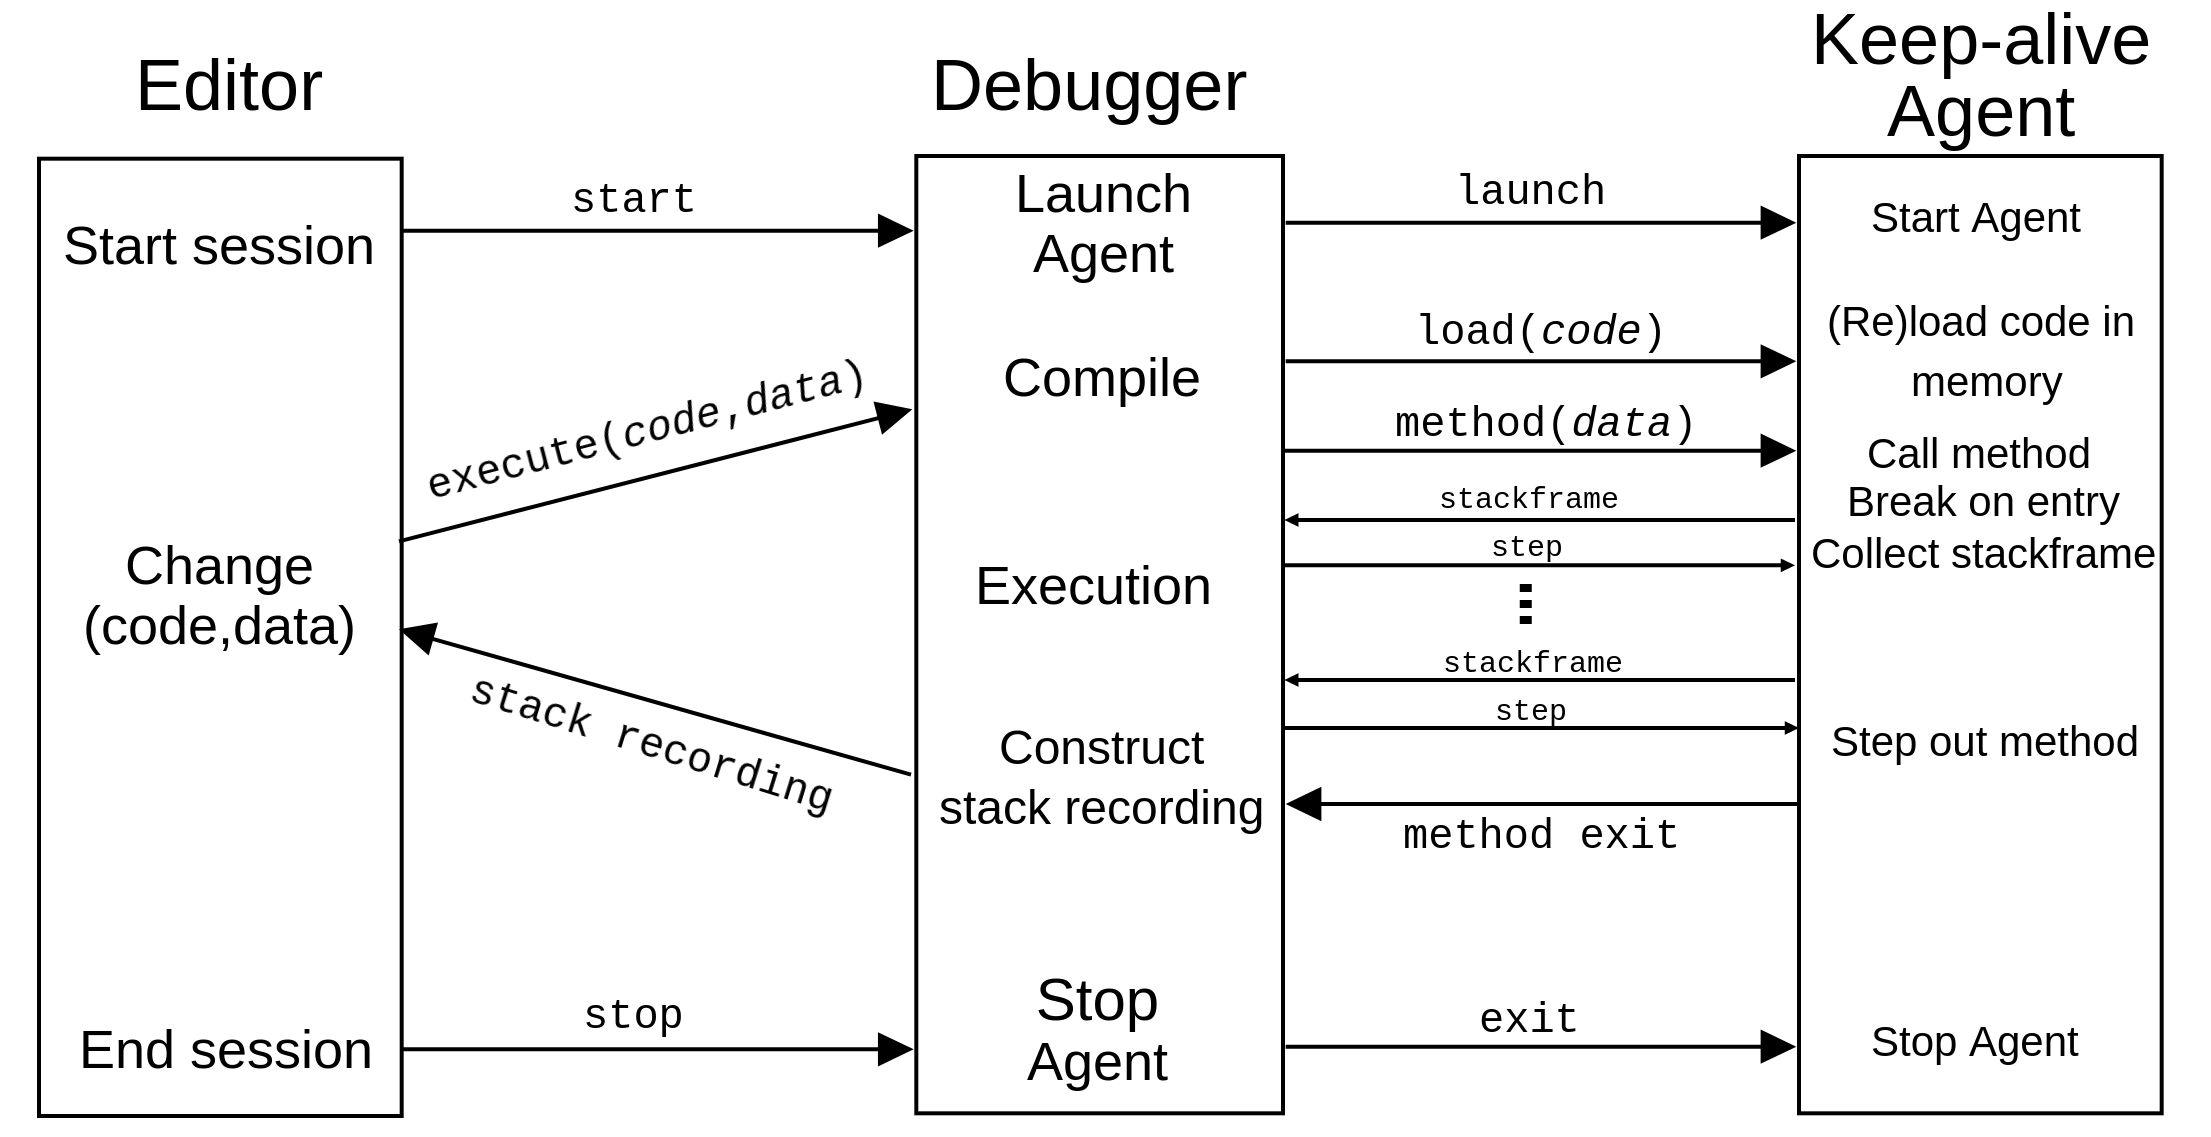
\includegraphics[width=0.8\linewidth]{img/keepalive_agent.png}
  \caption{Keep Alive Agent}
  \label{fig:keepalive-agent}
\end{figure}

A live environment must be able to react to two different events: a change in the code or a change in the test/input data. 
If the code changes, we need to re-execute the code, and in the case of a compiled language, we need to compile the new code first. 
If the data changes, we need to be able to re-execute the programme with the new data. 
In addition, it is necessary to keep compilation and execution times low enough to maintain an interactive experience with the user.

To meet these constraints, we propose to use the debugger on an intermediate program, a \textit{keep-alive agent}. 
This program keeps the debugger alive between executions and code changes to reduce initialisation times. 
The general operation of a keep-alive agent is shown in Figure \ref{fig:keepalive-agent} :
% TODO : make figure clean and add better description here
\begin{itemize}
  \item At the start of the session, the debugger is started on the agent. Once initialised, the agent is paused.
  \item The target code is loaded into the agent and a breakpoint is set at the input of the target method.
  \item Execution of the target method triggers the breakpoint at the input of the method, and execution continues step by step to build the \textit{stack recording}.
\end{itemize}

\section{Live Probes in Java with JDI}
\label{sec:live-probes-java}

We developed a Java backend using JDI, a debugging interface for Java, to implement the concepts discussed in the previous section. 
The keep-alive agent includes a method for loading classes into the JVM.

When executing the target method, the arguments are created in the client JVM and then passed to the debugger JVM using the \code{mirrorOf} and \code{newInstance} methods from the reflection API. 
The target method is invoked using \code{invokeMethod}. 
To handle events from the JDI when breakpoints are set, a dedicated thread is used to prevent deadlocks.

If modifications are needed in the code of the target method, we employ the \code{redefineClasses} method. 
This method allows changing the content of a class loaded in the JVM using an array of byte codes. 
However, it has a limitation: it only works if the class signature remains unchanged. 
If the class structure is modified, restarting the debugger is necessary.

\section{Generalizing Live Probes with Debugger Adapter Protocol}
\label{sec:generalizing-live-probes}
The Debug Adapter Protocol (DAP), developed by Microsoft, is a standard method of communicating with a programming language debugger. It is compatible with various editors, including VS Code, and provides a unified interface for all programming languages. 

By exploiting this protocol, we have created a new language parametric backend, which we have implemented for the C, Python and Java programming languages. These languages are chosen to cover both compiled and interpreted languages. 
This backend offers an interface common to all three languages, which includes methods for starting and initialising the debugging server, loading and reloading code in the debugger, and executing a method while performing stack recording. 

These methods allow us to carry out stack recording independently of the chosen language and facilitate the future implementation of live programming interfaces. 

The implementation for each language includes a keep-alive agent and code to communicate with the debugger and keep-alive agent to provide the interface functionality.
These methods depend on both the implementation of the debugging server and the keep-alive agent. 
The debug server initialisation parameters are specific to each language.

The way in which the code is loaded also depends on the language. 
For interpreted languages such as Python, the code can be interpreted at runtime and then loaded into the debugger's memory. 
For Java, we have extended the ClassLoader to add and modify classpaths and classes at runtime in the keep-alive agent. 
For C, the code is loaded into shared libraries that can be added and reloaded during execution.

Method execution for Java and Python is different to that used in C. 
For Java and Python, calling methods directly from the debugger does not trigger breakpoints for these languages. 
To remedy this, execution must be initiated from the agent and not by a debugger command. 
To do this, the Python and Java agents have fields for referencing a method and its arguments; when this information is entered, the agent starts execution.
For C, as is the case in the backend using JDI, the method call is made from the debugger console.

\section{Evaluation}
\label{sec:evaluation}
\subsection{Demo : A Minimal Live Programming Environment}
\label{sec:demo-small-c}
\begin{figure}[htbp]
  \centering
  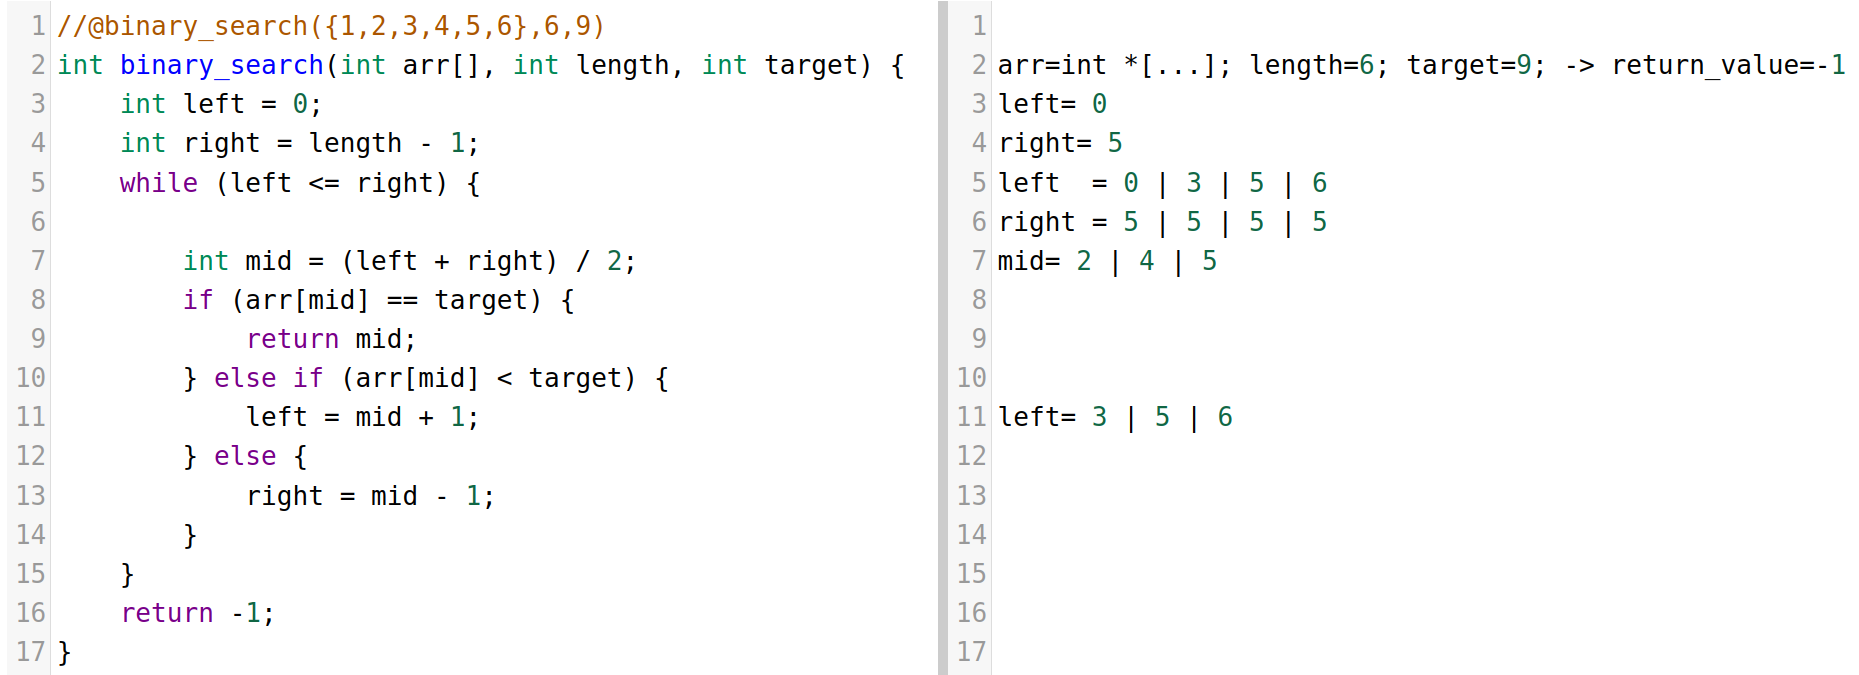
\includegraphics[width=\linewidth]{img/demo/c.png}
  \caption{Demo of the live programming environment for C.}
  \label{fig:demo}
\end{figure}

We have developed a dynamic programming environment that incorporates live probes through Java, C, and Python debug servers. 
The user interface consists of a web page that interacts with a local server. 
In Figure \ref{fig:demo}, we present a screenshot depicting a session with a binary\_search function in C. 
On the left-hand side, there is a code editor (based on CodeMirror 5), while on the right, a panel showcases live probes.

Whenever changes are made in the code editor, the code is sent to the server, which then checks for parseability and syntax errors. 
Additionally, if the code contains a comment starting with "@", followed by a function call, the server attempts to create a stack recording of that function, along with the provided parameters. 
This stack recording is subsequently processed through a parser to generate live probes, offering the following functionalities:

\begin{itemize}
  \item Displaying input arguments and return values for each function call.
  \item Showing the value of each variable definition or assignment. In cases where the assignment is within a loop or called multiple times, all the different values are displayed.
  \item Presenting the comparison values for each loop (for and while).
\end{itemize}
    
\subsection{Performance}
\label{sec:performance}

In the context of a live programming environment, it is essential to have short response times after user interactions. 
We therefore measured the performance of our approach in response to various questions:

\begin{itemize}
  \item How long does it take to compile and to load the code into the debugger, depending on the size of the programme?
  \item How long does it take to run the program, depending on the number of stack frames needed to make the stack recording?
  \item What is the average performance during a live programming session?
\end{itemize}

\subsubsection{How long does it take to compile and to load the code into the debugger, depending on the size of the programme?}

\begin{figure}[htbp]
  \centering
  \begin{subfigure}[b]{0.48\textwidth}
      \centering
      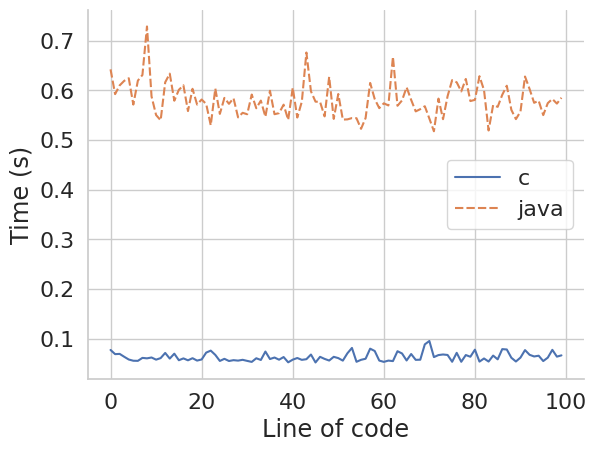
\includegraphics[width=\textwidth]{img/compile_code.png}
      \caption{\centering Compile code time}
      \label{subfig:compile}
  \end{subfigure}
  \hfill
  \begin{subfigure}[b]{0.48\textwidth}
      \centering
      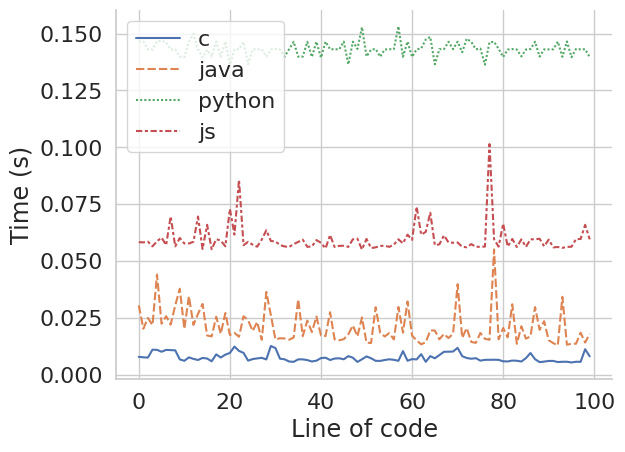
\includegraphics[width=\textwidth]{img/load_code.png}
      \caption{\centering Load code time}
      \label{subfig:load}
  \end{subfigure}
  \caption{Compile and load code time depending on the number of lines of code.}
  \label{fig:compileload}
\end{figure}

In our evaluation, we assessed the time required to compile and load code into the debugger memory for Python, C, and Java. 
To accomplish this, we compiled and loaded programs ranging from 5 to 100 lines of code. 
The summarized results can be found in Figure \ref{fig:compileload}.

In Sub-figure \ref{subfig:compile}, we present the compilation time for C and Java based on the number of lines of code. 
The compilation process was executed from the command line using javac and gcc. 
The compilation times remain nearly constant, regardless of the number of lines of code, with an average of 34.6 ms for Java and 8.5 ms for C.

Moving to Sub-figure \ref{subfig:load}, we depict the loading time in the debugger for C, Java, and Python as a function of the number of lines of code. 
The data shows that the loading time remains constant concerning the number of lines of code. 
On average, Python takes 3 ms, Java takes 2.8 ms, and C takes 1 ms for loading.

\subsubsection{How long does it need to run the program, depending on the number of steps to make the stack recording ?}

\begin{figure}[htbp]
  \centering
  \begin{subfigure}[b]{0.45\textwidth}
      \centering
      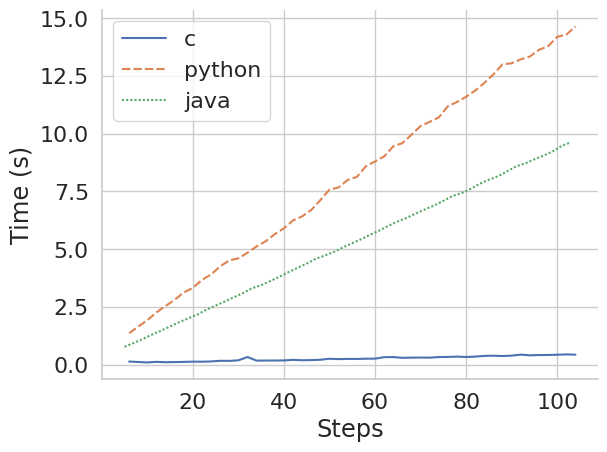
\includegraphics[width=\textwidth]{img/execute.png}
      \caption{\centering Total execution time}
      \label{subfig:execute-time-total}
  \end{subfigure}
  \hfill
  \begin{subfigure}[b]{0.45\textwidth}
      \centering
      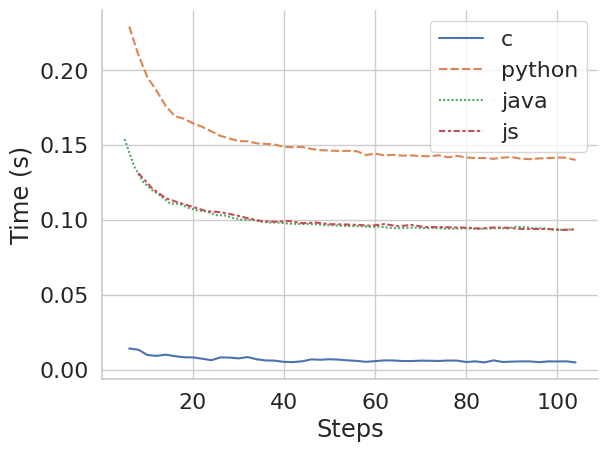
\includegraphics[width=\textwidth]{img/execute_ps.png}
      \caption{\centering Execution time per step}
      \label{subfig:execute-time-ps}
  \end{subfigure}
  \caption{Execution time in seconds depending on the number of steps.}
  \label{fig:execute-time}
\end{figure}

Subsequently, we proceeded to evaluate the execution time concerning the number of steps in the debugger. 
Figure \ref{subfig:execute-time-total} presents the total time taken based on the number of steps during stack recording, while Figure \ref{subfig:execute-time-ps} demonstrates the time per step as a function of the number of steps. 
Notably, the execution time exhibits a linear relationship with the number of steps in the method.

\subsubsection{What is the average performance during a live programming session?}

\begin{table}[h]
  \centering
  \begin{tabular}{@{} r c c c c c c c c c @{}}
  \toprule
  & \multicolumn{1}{c}{One time} & \multicolumn{3}{c}{Each Iteration} \\
  
  Language & Initialization & Compile & Load Code & Execute \\ \midrule
  C & 1.24 & 0.067 & 0.0098 & 0.193 \\
  Java & 5.92 & 0.57 & 0.015 & 1.28 \\
  Python & 0.639 & 0 & 0.144 & 3.26 \\
  \bottomrule
  \end{tabular}
  \caption{Average time in seconds for each step of the live programming session.}
  \label{table:average-time}
\end{table}

\begin{figure}[htbp]
  \centering
  \begin{subfigure}[b]{0.3\textwidth}
      \centering
      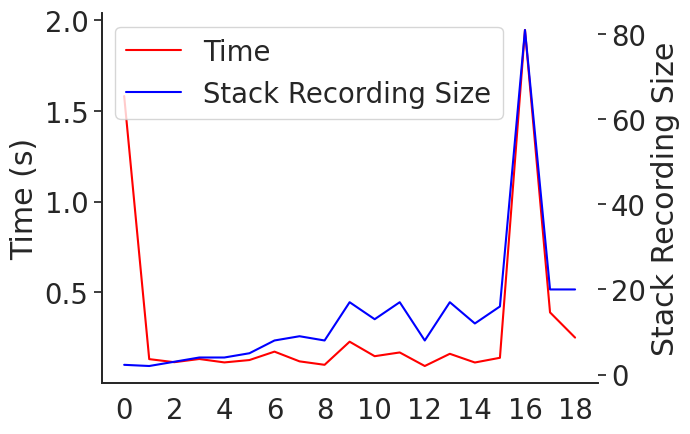
\includegraphics[width=\textwidth]{img/scenario_bs_c.png}
      \caption{\centering C}
      \label{subfig:scenario-bs-c}
  \end{subfigure}
  \hfill
  \begin{subfigure}[b]{0.3\textwidth}
      \centering
      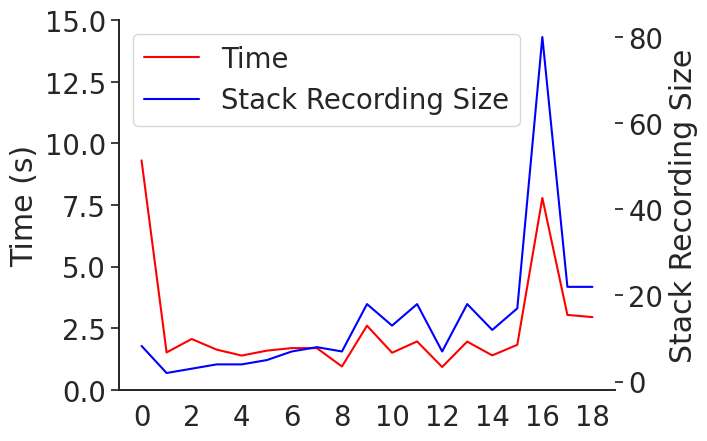
\includegraphics[width=\textwidth]{img/scenario_bs_java.png}
      \caption{\centering Java}
      \label{subfig:scenario-bs-java}
  \end{subfigure}
  \hfill
  \begin{subfigure}[b]{0.3\textwidth}
    \centering
    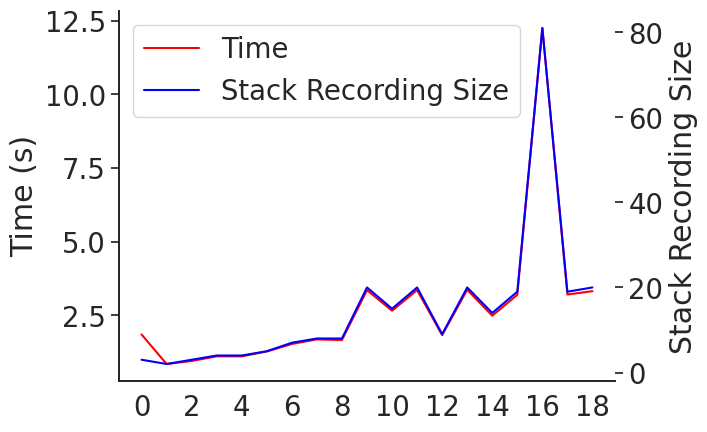
\includegraphics[width=\textwidth]{img/scenario_bs_python.png}
    \caption{\centering Python}
    \label{subfig:scenario-bs-py}
  \end{subfigure}

  \caption{Execution time and Stackrecording size for binary search scenario.}
  \label{fig:scenario-bs}
\end{figure}

To evaluate the performance of our approach in the general context of a live programming session, we measured the times taken by the different stages of the interaction loop:

\begin{itemize}
  \item Agent initialisation time, which occurs once at the start of the session.
  \item The compilation time, if there is a compilation stage.
  \item The time taken to load the code into the debugger.
  \item Program execution time.
\end{itemize}

For the 3 languages we have implemented, we have performed the measurements for the execution of a binary search function \ref{fig:binary-search}.
For each language, the agent was initialized, then the code was compiled, loaded into the debugger and executed (with the array [1,2,3,4,5,6] and target 9) 100 times.
Each execution generate a stack recording of approximately 20 stack frames.
The results are shown in table \ref{table:average-time}.





\section{Related Work}
\label{sec:related-work}

Example-Based Live Programming for Everyone\cite{10.1145/3426428.3426919} : Use GraalVM/Truffle to get live information from the code of multiple languages.

Example Centric Programming\cite{10.1145/1052883.1052894} : Use BeanShell(custom JVM) to get live information. Prototype for Java in Eclipse.

Usable Live Programming\cite{10.1145/2509578.2509585} : New language for live programming(Ying Yang) with incremental compilation. Live programming environment for this language.
Use source location to relate execution and code(=> almost like stack recording that link stackframe and code location)

Scalable Omniscient Debugging\cite{10.1145/1297105.1297067} : Omniscient debugging with a lot of data. Use a lot of memory to store all the data.
In this paper they record almost everything, we only record the stackframe.

\section{Conclusion}
\label{sec:conclusion}

\printbibliography

\newpage
\section*{Appendix}
\label{sec:appendix}

\begin{figure}[h]
  \centering
    \begin{lstlisting}[language=C]
int binary_search(int arr[], int length, int target) {
  int left = 0;
  int right = length - 1;
  while (left <= right) {

      int mid = (left + right) / 2;
      if (arr[mid] == target) {
          return mid;
      } else if (arr[mid] < target) {
          left = mid + 1;
      } else {
          right = mid - 1;
      }
  }
  return 0;
}
    \end{lstlisting}
  
    \begin{lstlisting}[language=Python]
def binary_search(arr, target):
    left = 0
    right = len(arr) - 1

    while left <= right:
        mid = (left + right) // 2

        if arr[mid] == target:
            return mid
        elif arr[mid] < target:
            left = mid + 1
        else:
            right = mid - 1

    return 0 
    \end{lstlisting}
 
    \begin{lstlisting}[language=Java]
public class BinarySearch {
    public static int binarySearch(int[] array, int key){
        int low = 0;
        int high = array.length - 1;
        while (low <= high) {
            int mid = (low + high) / 2;
            int value = array[mid];
            if (value < key) {
                low = mid + 1;
            } else if (value > key) {
                high = mid - 1;
            } else {
                return mid;
            }
        }
        return 0;
    }
}
      \end{lstlisting}
  \caption{Binary Search in C, Python and Java}
  \label{fig:binary-search}
\end{figure}



\end{document}

% Local Variables:
% TeX-engine: luatex
% End:
